%% Homework 5 - Tate Mason %%
\documentclass[10pt, a4paper]{article}
\usepackage[top=3cm, bottom=4cm, left=3.5cm, right=3.5cm]{geometry}
\usepackage{amsmath,amsthm,amsfonts,amssymb,amscd, fancyhdr, color, comment, graphicx, environ}
\usepackage{float}
\usepackage{mathtools}
\usepackage{mathrsfs}
\usepackage[math-style=ISO]{unicode-math}
\DeclareSymbolFont{\mathnormal}{letters}
\usepackage{lastpage}

%%%%%%%%%%%%%%%%%%%%%%%%%%%%%%%%%%%%%%%%%%%%%%%%%%%%%%%%%%%%%%%%%%
%%%%%%%%%%%%%%%%%%%%%%%%%%%%%%%%%%%%%%%%%%%%%%%%%%%%%%%%%%%%%%%%%%
%Fill in the appropriate information below
\newcommand{\norm}[1]{\left\lVert#1\right\rVert}     
\newcommand\course{ECON - 8010}                            % <-- course name   
\newcommand\hwnumber{ 5}                                 % <-- homework number
\newcommand\Information{Tate Mason}                        % <-- personal information
%%%%%%%%%%%%%%%%%%%%%%%%%%%%%%%%%%%%%%%%%%%%%%%%%%%%%%%%%%%%%%%%%%
%%%%%%%%%%%%%%%%%%%%%%%%%%%%%%%%%%%%%%%%%%%%%%%%%%%%%%%%%%%%%%%%%%
%Page setup
\pagestyle{fancy}
\headheight 35pt
\lhead{\today}
\rhead{}
\lfoot{}
\pagenumbering{arabic}
\cfoot{\small\thepage}
\rfoot{}
\headsep 1.2em
\renewcommand{\baselinestretch}{1.25}
%%%%%%%%%%%%%%%%%%%%%%%%%%%%%%%%%%%%%%%%%%%%%%%%%%%%%%%%%%%%%%%%%%
%%%%%%%%%%%%%%%%%%%%%%%%%%%%%%%%%%%%%%%%%%%%%%%%%%%%%%%%%%%%%%%%%%
%Add new commands here
\renewcommand{\labelenumi}{\alph{enumi})}
\newcommand{\var}{\text{var}}
\newcommand{\Z}{\mathbb Z}
\newcommand{\R}{\mathbb R}
\newcommand{\Q}{\mathbb Q}
\newcommand{\NN}{\mathbb N}
\newcommand{\PP}{\mathbb P}
\DeclareMathOperator{\Mod}{Mod} 
\renewcommand\lstlistingname{Algorithm}
\renewcommand\lstlistlistingname{Algorithms}
\def\lstlistingautorefname{Alg.}
\newtheorem*{theorem}{Theorem}
\newtheorem*{lemma}{Lemma}
\newtheorem{case}{Case}
\newcommand{\assign}{:=}
\newcommand{\infixiff}{\text{ iff }}
\newcommand{\nobracket}{}
\newcommand{\backassign}{=:}
\newcommand{\tmmathbf}[1]{\ensuremath{\boldsymbol{#1}}}
\newcommand{\tmop}[1]{\ensuremath{\operatorname{#1}}}
\newcommand{\tmtextbf}[1]{\text{{\bfseries{#1}}}}
\newcommand{\tmtextit}[1]{\text{{\itshape{#1}}}}

\newenvironment{itemizedot}{\begin{itemize} \renewcommand{\labelitemi}{$\bullet$}\renewcommand{\labelitemii}{$\bullet$}\renewcommand{\labelitemiii}{$\bullet$}\renewcommand{\labelitemiv}{$\bullet$}}{\end{itemize}}
\catcode`\<=\active \def<{
\fontencoding{T1}\selectfont\symbol{60}\fontencoding{\encodingdefault}}
\catcode`\>=\active \def>{
\fontencoding{T1}\selectfont\symbol{62}\fontencoding{\encodingdefault}}
\catcode`\<=\active \def<{
\fontencoding{T1}\selectfont\symbol{60}\fontencoding{\encodingdefault}}

%%%%%%%%%%%%%%%%%%%%%%%%%%%%%%%%%%%%%%%%%%%%%%%%%%%%%%%%%%%%%%%%%%
%%%%%%%%%%%%%%%%%%%%%%%%%%%%%%%%%%%%%%%%%%%%%%%%%%%%%%%%%%%%%%%%%%
%Begin now!

\begin{document}
  \begin{titlepage}
    \begin{center}
      \vspace*{3cm}
            
        \vspace{1cm}
        \huge
        Homework \hwnumber
            
        \vspace{1.5cm}
        \Large
            
        \textbf{\Information}                      % <-- author
            
        \vfill
        
        An \course \ Homework Assignment
            
        \vspace{1cm}
        \Large

        
        \today
            
    \end{center}
  \end{titlepage}

  \newpage
\section*{PS1 - Question 3}
  \subsection*{Problem}
    In a second-price auction, each of the n bidders simultaneously places a bid for an
    object. The object is won by the bidder with the highest bid, who pays the amount of
    the second-highest bid. If there are multiple highest bids, then the winner is chosen at random from among the highest bidders, and this winner pays the highest bid (since this is also the second-highest bid).

    Suppose that player i values the object at vi dollars, and that all players’ valuations are commonly known. Show that it is a weakly dominant strategy for player i to bid his valuation.
  \subsection*{Solution}
\section*{PS1 - Question 4}
  \subsection*{Problem}
    Two travelers returning home from a remote island where they bought identical antiques discover that the airline has managed to smash them. The airline manager decides to use the following scheme to determine the compensation that the airline will give each traveler: Each traveler will separately report the cost of the antique, stating an integer number of dollars between 2 and 500. If both report the same number of dollars, then the airline will give each of them that number of dollars. If they report different numbers of dollars, then the traveler who stated the smaller number will be given the amount he stated plus a bonus of 2 dollars; the traveler who stated the higher number will be given the amount stated by the other traveler minus a penalty of 2 dollars. Suppose that each traveler cares only about maximizing the expected number of dollars he receives from the airline.
    \subsubsection*{(i)}
      Define the normal form game $G$ corresponding to the story above specifying the set of players $\mathcal{P}$, their strategy sets  $S_i$, and their payoff functions $u_i$.
    \subsubsection*{(ii)}
      Fix player 1's beliefs $\mu_1\in\Delta S_2$, ans suppose that the highest strategy in $S_2$ that receives positive probability under $\mu_1$ is $\bar{s}_2>2$. Show that player 1's best response given his beliefs must be less than $\bar{s}_2$. (Hint: Start by computing player 1's payoff from choosing a strategy greater than $\bar{s}_2$, and notice that answering the question does not necessarily require you to compute player 1's best response to $\mu_1$)
    \subsubsection*{(iii)}
      If there is a common knowledge of rationality between the players, what is the appropriate prediction of play in $G$?
  \subsection*{Solutions}
    \subsubsection*{(i)}
      \begin{gather*}
        $\mathcal{P} = \{1,2\}$\\
        $S_i \in [2,500]$ \\ 
        \text{Payoffs:}\\
          s_1 = s_2: u(s_1, s_2) = s_i \ for \ i \in [1,2] \\
          s_1 > s_2: u(s_1, s_2) = s_2 - 2 \\
          s_1 < s_2: u(s_1, s_2) = s_1 + 2 \\
      \end{gather*}
\section*{PS1 - Question 5}
  \subsection*{Problem}
    Consider the following normal form game:
    \begin{center}
      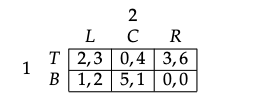
\includegraphics[width = 0.4\textwidth]{PS1-5.png}
    \end{center}
    \subsubsection*{(i)}
      Are any pure strategies in this game strictly dominated? If so, then for each such strategy $s_i$, identify all dominating strategies that do not put positive probability on $s_i$.
    \subsubsection*{(ii)}
      If there is common knowledge of rationality between the players, what should our prediction of play in this game be?
\section*{PS1 - Question 7}
  \subsection*{Problem}
    Which pure strategies are rationalizable in the following normal form game? Explain.
    \begin{center}
      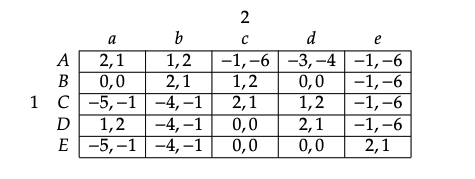
\includegraphics[width = 0.72\textwidth]{PS1-7.png}
    \end{center}
\section*{PS2 - Question 1}
  \subsection*{Problem}
    Compute all Nash equilibria in the following game:
    \begin{center}
      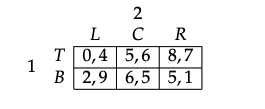
\includegraphics[width = 0.4\textwidth]{PS2-1.png}
    \end{center}
\section*{PS2 - Question 2}
  \subsection*{Problem}
    Find all Nash equilibria in the following game: 
    \begin{center}
      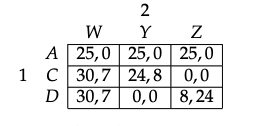
\includegraphics[width=0.4\textwidth]{PS2-2.png}
    \end{center}
\end{document}

